\documentclass[../notes.tex]{subfiles}

\pagestyle{main}
\renewcommand{\chaptermark}[1]{\markboth{\chaptername\ \thechapter\ (#1)}{}}
\setcounter{chapter}{5}

\begin{document}




\chapter{Magnetochemistry}
\section{Magnetochemistry I}
\begin{itemize}
    \item \marginnote{2/7:}Extension of last time's material: The derivation of the relationship for the between spring harmonic oscillator frequencies and the oscillators' reduced masses.
    \begin{itemize}
        \item Suppose you have two homonuclear diatomic molecules \ce{A-A} and \ce{B-B}, and you wish to relate their vibrational frequencies.
        \item Reduced masses of the molecules.
        \begin{align*}
            \mu_{\ce{AA}} &= \frac{m_{\ce{A}}m_{\ce{A}}}{m_{\ce{A}}+m_{\ce{B}}}&
            \mu_{\ce{BB}} &= \frac{m_{\ce{B}}m_{\ce{B}}}{m_{\ce{B}}+m_{\ce{B}}}
        \end{align*}
        \item Vibrational frequencies of the molecules in terms of the reduced masses.
        \begin{align*}
            \nu_{\ce{AA}} &= k\sqrt{\frac{F}{\mu_{\ce{AA}}}}&
            \nu_{\ce{BB}} &= k\sqrt{\frac{F}{\mu_{\ce{BB}}}}
        \end{align*}
        \item Take the ratio of the above two quantities to relate them.
        \begin{equation*}
            \frac{\nu_{\ce{AA}}}{\nu_{\ce{BB}}} = \frac{k\sqrt{\frac{F}{\mu_{\ce{AA}}}}}{k\sqrt{\frac{F}{\mu_{\ce{BB}}}}}
            = \frac{\sqrt{\mu_{\ce{BB}}}}{\sqrt{\mu_{\ce{AA}}}}
        \end{equation*}
    \end{itemize}
    \item Anything else I missed??
    \item Today: Magnetochemistry.
    \begin{itemize}
        \item 1-2 lectures on this.
        \item \textcite{bib:CHEM20100Notes} has a good write-up of the derivation at the beginning of today's lecture (see Module 34: Magnetic Properties of Transition Metal Complexes), and \textcite{bib:CHEM20200Notes} has more on the content at the end of the lecture (see Lecture 3: TM Magnetism).
    \end{itemize}
    \item Magnetism really is the province of inorganic chemistry since it's here that we find the compounds with unpaired electrons.
    \begin{itemize}
        \item Organic compounds don't have these outside of free radicals.
    \end{itemize}
    \item The nuclei interact with...??
    \item \textbf{Magnetic field}. \emph{Denoted by} $\bm{H}$, $\bm{\vec{H}}$.
    \begin{itemize}
        \item $H$ denotes the magnitude of $\vec{H}$.
    \end{itemize}
    \item \textbf{Magnetization}: The response of a material to a magnetic field. \emph{Denoted by} $\bm{M}$.
    \begin{itemize}
        \item Alternatively: The magnetic moment per unit volume.
        \item Everything with electrons has \emph{some} degree of a response to a magnetic field.
    \end{itemize}
    \item \textbf{Magnetic induction}: The density of magnetic field lines within a substance. \emph{Denoted by} $\bm{B}$. \emph{Units} Teslas or Gauss.
    \begin{itemize}
        \item $\SI{1}{\tesla}=\SI{10000}{\gauss}$.
        \item The scale of these units.
        \begin{itemize}
            \item The Earth's magnetic field is about \SI{3e-5}{\tesla}.
            \item A \SI{900}{\mega\hertz} NMR spectrometer is about \SI{21}{\tesla}.
            \item An MRI is about \SIrange{1.3}{3}{\tesla}.
        \end{itemize}
        \item Additionally, $B=F/Qv$ where $F$ is in Newtons, $Q$ is in Coulombs, and $v$ is in meters per second.
    \end{itemize}
    \item Placing a sample with magnetization $M$ in a magnetic field $\vec{H}$ alters the magnetic induction via
    \begin{equation*}
        B = \vec{H}+4\pi\vec{M}
    \end{equation*}
    \item The force that an object in a magnetic fields feels is
    \begin{equation*}
        \vec{f} = \vec{M}\cdot\dv{H}{z}
    \end{equation*}
    \item \textbf{Magnetic susceptibility}. \emph{Denoted by} $\bm{\chi}$. \emph{Given by}
    \begin{equation*}
        \chi = \frac{\vec{M}}{\vec{H}}
    \end{equation*}
    \begin{itemize}
        \item A tensor of rank 2.
        \item It follows that $\vec{M}=\vec{\chi}\vec{H}$.
    \end{itemize}
    \item \textbf{Volume susceptibility}: \emph{Denoted by} $\bm{\chi_V}$. \emph{Units} \si{\electromagneticunits\per\cubic\centi\meter}.
    \item \textbf{Gram susceptibility}: \emph{Denoted by} $\bm{\chi_g}$. \emph{Units} \si{\cubic\centi\meter\per\gram}. \emph{Given by}
    \begin{equation*}
        \chi_g = \frac{\chi_V}{d}
    \end{equation*}
    \item \textbf{Molar susceptibility}: \emph{Denoted by} $\bm{\chi_M}$. \emph{Units} \si{\cubic\centi\meter\per\mole}. \emph{Given by}
    \begin{equation*}
        \chi_m = \chi_g\cdot\text{MW}
    \end{equation*}
    \item $\chi>0$ indicates unpaired electrons. $\chi<0$ indicates paired electrons.
    \item Diamagnetism
    \item Most matter is diamagnetic.
    \item \textbf{Gouy balance}: An instrument that measures the change in mass of a sample as it is attracted ore repelled by a powerful magnetic field.
    \begin{figure}[h!]
        \centering
        \begin{tikzpicture}
            \footnotesize
            \draw (-1.5,0) -- ++(1,0) -- node[left]{$N$} ++(0,0.5) -- ++(-1,0);
            \draw (1.5,0) -- ++(-1,0) -- node[right]{$S$} ++(0,0.5) -- ++(1,0);
            \draw [dashed] (-0.5,0.25) -- ++(1,0);
    
            \draw [semithick,-latex] (0,0.8) -- ++(0,-1);
            \fill [blx!20] (-0.1,1) -- (-0.1,0.8) to[out=-90,in=-90,looseness=2] (0.1,0.8) -- (0.1,1) -- cycle;
            \draw [gray,thick] (-0.1,1.5) -- (-0.1,0.8) to[out=-90,in=-90,looseness=2] (0.1,0.8) -- (0.1,1.5) -- cycle;
            \draw (0,1.5) -- ++(0,0.5) -- ++(1,0) -- ++(0,-0.3) node[below]{scale};
        \end{tikzpicture}
        \caption{Gouy balance.}
        \label{fig:Gouy}
    \end{figure}
    \begin{itemize}
        \item Historically, varying a magnetic field precisely has been very difficult (we didn't always have electromagnets into which we could just dial any field).
        \begin{itemize}
            \item In fact, even today, varying a magnetic field super precisely is difficult. This is why NMR machines vary the frequency domain over a constant magnetic field.
        \end{itemize}
        \item Under this constant magnetic field, we linked a sample to a scale. As we move our sample through that field, we have a changing magnetic field.
        \item How the mass of the sample changes at different points in the field gives information on the magnetic susceptibility.
    \end{itemize}
    \item Modern update to the Gouy balance: The superconducting quantum interference device, or SQUID.
    \begin{itemize}
        \item We still measure the magnetic susceptibility essentially the same way, just with fancier toys.
        \item Today, we move our sample through an electromagnet-generated magnetic field and then see what kind of current gets induced in a superconducting coil (recall that moving magnets induces currents).
        \item The underlying physics is well beyond the scope of this course, but also fascinating. It involves \textbf{Josephson junctions}, etc.
    \end{itemize}
    \item \textbf{Diamagnetic magnetic susceptibility}. \emph{Denoted by} $\bm{\chi_\textbf{dia}}$.
    \item Per the above, since all electrons are paired in a diamagnetic compound, $\chi_\text{dia}<0$.
    \item We have
    \begin{equation*}
        \chi_\text{dia} = \sum\lambda+\sum n_i\chi_i
    \end{equation*}
    \begin{itemize}
        \item $\lambda$ is a \textbf{constitutive correction} related to ring currents for bonds.
        \item $n_i\chi_i$ is contributions from individual atoms.
    \end{itemize}
    \item Info on the quantities in the above equations can be found in \textcite{bib:BerryDiamagnetism}.
    \begin{itemize}
        \item The paper has a nice introduction and does the derivation that Anderson just did, too.
        \item Then it contains a bunch of tables of different corrections for various bond types.
        \item These values are all pretty small, so it doesn't really matter if you just miss one or two things in ambiguous cases, but Anderson tries to sum over all of them.
        \item You need to do these corrections when you're doing a lot of these calculations.
        \item These tables give both $\lambda$ and $\chi_i$ values; you need to sum over the individual atom $\chi_i$ values and then constitutive corrections for groups. For example, for a \ce{Cp} group, you have 5 carbons, 5 hydrogens, and a constitutive correction for the whole group (which should be equal to that of 5 carbons, 5 hydrogens, and 5 \ce{C=C} double bonds??).
        \item These values are field-independent and pretty constant.
    \end{itemize}
    \item That's the contribution from paired electrons. What we really care about in general are the unpaired electrons, though.
    \item Paramagnetism.
    \item Paramagnets.
    \begin{itemize}
        \item Positive $\chi$ values. The substance will be pulled into the magnetic field.
        \item Inversely proportional relationship between $\chi$ and $T$ so that $1/\chi$ vs. $T$ is linear.
        \item Implies \textbf{Curie's law}, where $\chi=C/T$ and $C$ is the Curie constant.
        \begin{equation*}
            C = \frac{\NA g^2\mB(S(S+1))}{3\kB (in hertz??)}
        \end{equation*}
        \item $g$ is the \textbf{gyromagnetic ratio} and, occasionally, some other names for added complexity :)
        \item $\mB$ is the Bohr magneton.
        \item $\NA$ is Avogadro's number.
        \item $S$ is our spin quantum number.
    \end{itemize}
    \item \textbf{Gyromagnetic ratio}: The quotient of the magnetic moment by the angular momentum. \emph{Also known as} \textbf{magnetogyric ratio}. \emph{Denoted by} $\bm{g}$.
    \begin{itemize}
        \item Any fundamental particle can have one of these.
        \item Nuclei have them, but we're only worried about electrons here.
        \item Magnetic moment divided by angular momentum.
        \item 2.011 for electrons.
    \end{itemize}
    \item We want to take this picture and simplify it down now.
    \item We have
    \begin{equation*}
        \mu_\text{eff} = \sqrt{\frac{\kB}{\NA\mB^2}}\sqrt{\chi T}
        = 2.828\sqrt{\chi T}
        = \sqrt{g^2(S(S+1))}
    \end{equation*}
    \item $\mu_\text{eff}=\sqrt{g^2(S(S+1))}$, $\chi T=g^2/8$ are our big results.
    \item We also frequently write
    \begin{equation*}
        \chi T = \frac{\NA g^2\mB}{3\kB}(S(S+1))
        = \frac{g^2}{8}(S(S+1))
    \end{equation*}
    \item Magnetochemists will almost exclusively use $\chi T$, but you see $\mu_\text{eff}$ reported a lot, especially for room temperature characteriztions.
    \item Know the two end results below because they're very important for how stuff is computed and talked about in the literature.
    \begin{align*}
        \mu_\text{eff} &= \sqrt{g^2(S(S+1))}&
        \chi T &= \frac{g^2}{8}S(S+1)
    \end{align*}
    \item Elements vs. their spin quantum numbers. Find the number of unpaired electrons and go from there.
    \begin{table}[h!]
        \centering
        \small
        \renewcommand{\arraystretch}{1.2}
        \begin{tabular}{c|cccc}
             & $S$ & $\mu_\text{eff}$ & $\chi T_{SO}$ & $\mu_\text{exp}$\\
            \hline
            \ce{Cu^2+} & 1/2 & 1.73 & 0.375 & \numrange{1.7}{2.2}\\
            \ce{Ni^2+} & 1 & 2.83 & 1 & \numrange{2.8}{3.5}\\
            \ce{Cr^3+} & 3/2 & 3.87 & 1.875 & \numrange{3.7}{3.9}\\
            \ce{Fe^2+} HS & 2 & 4.90 & 3 & \numrange{5.1}{5.7}\\
            \ce{Fe^3+} HS & 5/2 & 5.92 & 4.375 & \numrange{5.7}{6}\\
        \end{tabular}
        \caption{Magnetic parameters for example elements.}
        \label{tab:exampleElementsMagnetism}
    \end{table}
    \begin{itemize}
        \item SO for spin only. HS for high spin. exp for experimental.
    \end{itemize}
    \item Spin-orbit coupling: $g>0$ for a more than half-filled shell; $g<0$ for a less than half-filled shell.
    \item Consider a generic metal \ce{M} with $S=1/2$ and another with $S=1/2$ and a bridging ligand \ce{L} between them.
    \item Three possibilities to determine magnetism: The spins can be coupled antiferromagnetically (opposite directions) so $S=0$, feromagnetically coupled ($S=1$), and uncoupled (both behave as their own spin center but are chemically/mechanically linked within the molecule).
    \item Now switch to having \ce{Cu-L-Mn} to have $S=1/2$ and $S=5/2$. Then
    \begin{equation*}
        \prb{\mu} = \sqrt{\mu_{\ce{M}_1}^2+\mu_{\ce{M}_2}^2}
        = \sqrt{3+35}
        = 6.16\mB
    \end{equation*}
    \begin{itemize}
        \item How does this work?? What is $\prb{\mu}$?
        \item Alternatively, $\chi T$ can be calculated.
    \end{itemize}
    \item Temperature-independent paramagnetism.
    \begin{itemize}
        \item If we measure \ce{Cu^{II}} and \ce{Co^{II}}, we get \SI{60e-6}{emu} and \SI{400e-6}{emu}.
        \item Correcting Curie's law with the \textbf{Curie-Weiss law}
        \begin{equation*}
            \chi = \frac{C}{T-\theta}
        \end{equation*}
        where $\theta=0$ for a pure paramagnet and $\theta\neq 0$ for a long range magnetic interaction.
        \item Magnetic measurements are very sensitive; any time you're not fitting the data, 90\% of the time it's that your sample isn't clean.
    \end{itemize}
    \item Spin-orbit coupling is up next.
    \item $S$ is our spin angular momentum quantum number, and $L$ is our orbital angular momentum quantum number.
    \item We define $J=L+S$ to characterize coupling. $J$ is very important with the lanthanides where our coupling is extremely large. So strong that you have to start with only a $J$ quantum number. For first-row transition metals, we treat $J$ just as a perturbation.
    \item We know that $L=\sum_i\ell_i$ and $S=\sum_is_i$. Our Hamiltonian is
    \begin{equation*}
        H = \hat{H}_0+\hat{H}_\text{elec}+\hat{H}_\text{SO}
    \end{equation*}
    where SO denotes spin-orbit here and
    \begin{equation*}
        \hat{H}_{SO} = \lambda\hat{L}\cdot\hat{S}+\beta(\hat{L}+g_e\hat{S})-H
    \end{equation*}
    \item The energy that we get out of this Hamiltonian is
    \begin{equation*}
        E_n = E_n^0+HE_n^1+H^2E_n^2
    \end{equation*}
    \begin{itemize}
        \item The first-order correction is Zeeman; the second-order is 2nd order Zeeman.
    \end{itemize}
    \item Consider a perfectly octahedral $d^1$ complex. The electron can migrate through a degenerate set of orbitals, inducing a ring current. This is a useful classical analogy with predictive power; however, it is not quantum mechanically accurate at all.
    \item In a nutshell, we expect to see SO-coupling when we have unequally occupied degenerate orbitals.
    \begin{itemize}
        \item Consider \ce{Ni^2+}. It can be $O_h$ or $T_d$. It's tetrahedral because \ce{Ni^2+} is $d^8$ and thus if you draw out the orbital diagram, we'll have one excess electron in the upper triply degenerate orbital. This unequal occupation will lead to a Jahn-Teller distortion, though.
    \end{itemize}
    \item Free atom configurations are not a real thing; in this class, we'll always assume that transition metals are realistic, i.e., elemental, in a compound, etc., and thus any higher-level $s$ electrons fall down to $d$ electrons.
    \item Lanthanides' bonding orbitals are too deeply buried.
    \item \textbf{Zero-field splitting}: A difference in energy between "degenerate" electronic energy levels even in the presence of zero magnetic field. \emph{Denoted by} $\bm{D}$.
    \begin{figure}[h!]
        \centering
        \footnotesize
        \begin{subfigure}[b]{0.49\linewidth}
            \centering
            \begin{tikzpicture}[
                every node/.style={black}
            ]
                \draw (0,3) node[above]{\small$E$} -- (0,0) node[below right]{0} -- (4,0) node[below left]{$\infty$} node[right]{\small$H$};
    
                \draw [blx,ultra thick] (0,1.5) node[left]{$M_S=\pm\frac{1}{2}$} -- ++(0.5,0);
                \draw [blx,semithick]
                    (0.5,1.5) -- ++(2,0.7)
                    (0.5,1.5) -- ++(2,-0.7)
                ;
    
                \path (-1.8,0) -- (5.8,0);
            \end{tikzpicture}
            \caption{$S=1/2$, $D=0$.}
            \label{fig:zeroFieldSplita}
        \end{subfigure}
        \begin{subfigure}[b]{0.49\linewidth}
            \centering
            \begin{tikzpicture}[
                every node/.style={black}
            ]
                \draw (0,3) node[above]{\small$E$} -- (0,0) node[below right]{0} -- (4,0) node[below left]{$\infty$} node[right]{\small$H$};
    
                \draw [blx,ultra thick] (0,1.5) node[left]{$M_S=0,\pm 1$} -- ++(0.5,0);
                \draw [blx,semithick]
                    (0.5,1.5) -- ++(2,1.4)
                    (0.5,1.5) -- ++(2,0)
                    (0.5,1.5) -- ++(2,-1.4)
                ;
    
                \path (-1.8,0) -- (5.8,0);
            \end{tikzpicture}
            \caption{$S=1$, $D=0$.}
            \label{fig:zeroFieldSplitb}
        \end{subfigure}\\[1em]
        \begin{subfigure}[b]{0.49\linewidth}
            \centering
            \begin{tikzpicture}[
                every node/.style={black}
            ]
                \draw (0,3) node[above]{\small$E$} -- (0,0) node[below right]{0} -- (4,0) node[below left]{$\infty$} node[right]{\small$H$};
    
                \draw [blx,ultra thick] (0,2) node[left]{$M_S=\pm 1$} -- ++(0.5,0);
                \draw [blx,ultra thick] (0,1.5) node[left]{$M_S=0$} -- ++(0.5,0);
                \draw [blx,semithick]
                    (0.5,2) -- ++(2,0.7)
                    (0.5,2) -- ++(2,-0.7)
                    (0.5,1.5) -- ++(2,0)
                ;
    
                \draw [<->,shorten <=1pt,shorten >=1pt] (0.25,1.5) -- node[right]{$D$} ++(0,0.5);
    
                \path (-1.8,0) -- (5.8,0);
            \end{tikzpicture}
            \caption{$S=1$, $D\neq 0$.}
            \label{fig:zeroFieldSplitc}
        \end{subfigure}
        \caption{Zero field splitting.}
        \label{fig:zeroFieldSplit}
    \end{figure}
    \begin{itemize}
        \item Important for Qbits or more exotic materials.
        \item Look at graphs of energy as a function of applied magnetic field $H$ (see Figure \ref{fig:zeroFieldSplit}).
        \item We get Zeeman splitting as we increase the magnetic field. In the $D=0$ case, our splitting begins from a single point as in Figures \ref{fig:zeroFieldSplita}-\ref{fig:zeroFieldSplitb}.
        \item In Figure \ref{fig:zeroFieldSplitc}, however, we can observe splitting even at $H=0$.
        \item $D$ is on the order of single wavenumbers.
        \item Affects what EPR values you can excite and other important things. The $M_s=0$ state is still a triplet with parallel or antiparallel spins.
    \end{itemize}
\end{itemize}



\section{Magnetochemistry II}
\begin{itemize}
    \item \marginnote{2/9:}We just about wrapped up molecular magnetism last time.
    \item There are notes posted online for all of the lectures.
    \item Today: Materials magnetism.
    \item We start with some review from last time and lead into new content from there.
    \item Classical example of zero-field splitting for an $S=1$ compound.
    \begin{itemize}
        \item We have $M_s=-1,0,1$.
        \item The magnitude of spin-orbit coupling determines zero-field splitting.
        \item $D$ can be both positive and negative, so it can vary whether the higher state goes up or the lower state goes down. The short answer is just that splitting occurs.
        \item Recent example from the literature (unpublished): An aryl-bismuth compound with $S=1$ and massive $D\approx\SI{500}{\per\centi\meter}$. Another one is \ce{Bi-Bi^2-}.
    \end{itemize}
    \item Coupling.
    \begin{itemize}
        \item Electrons can couple parallel (FM --- ferromagnetic) or antiparallel (AF --- antiferromagnetic).
        \begin{itemize}
            \item Relevant Hamiltonian: The \textbf{Heisenberg-Dirac-Van Vleck Hamiltonian}.
        \end{itemize}
        \item We measure coupling by measuring $\chi$ vs. $T$.
        \begin{itemize}
            \item FM systems: As temperature decreases, $\chi$ slightly increases until the \textbf{Curie/critical temperature} $T_C$. At this point, the curve turns upwards sharply. For a bulk compound, the curve peaks at $T_C$ and then goes down.
            \item AM systems: As temperature decreases, there is a similar rise to a peak (this time at the \textbf{Neel temperature} $T_N$) and drop.
            \item As $J$ gets larger, the FM curve increases (i.e., $\chi$ increases). On the other hand, the AF curve decreases and flattens.
            \item See Figure 1.13 of \textcite{bib:CHEM20200Notes} and the picture from class.
        \end{itemize}
    \end{itemize}
    \item \textbf{Heisenberg-Dirac-Van Vleck} (Hamiltonian): The Hamiltonian defined as follows. \emph{Given by}
    \begin{equation*}
        \hat{H}_\text{HDVV} = -2J\cdot\vec{S}_1\cdot\vec{S}_2
    \end{equation*}
    \begin{itemize}
        \item $J$ is the coupling constant in \si{\per\centi\meter}.
    \end{itemize}
    \item \textbf{Bleaney-Bowers equation}: The equation describing the shape of the $\chi$ vs. $T$ plot for two spin centers of $S=1/2$. \emph{Given by}
    \begin{equation*}
        \chi = \frac{N\beta^2g^2}{3\kB T}\cdot\frac{3}{3+\e[2J/\kB T]}
    \end{equation*}
    \begin{itemize}
        \item Fitting data to this functional form allows you to pull out a value of $J$.
        \item Works best for two spin centers of $S=1/2$.
        \item There are softwares to do this fitting such as Dave (contact Anderson if you need it).
        \item Which of the previously discussed plots (FM/AM and bulk/molecular) can we fit with this equation?? Also check the functional form --- 2 in the numerator and negative sign in the exponent?
    \end{itemize}
    \item Orbital interactions for coupling.
    \begin{itemize}
        \item First system: Picture two spin centers $\ce{A},\ce{B}$ coupled with some diamagnetic bridging ligand \ce{X} such that we have \ce{A-X-B}.
        \item The only structure we assert is an orbital $\phi_{\ce{A}}$ on \ce{A} and likewise on \ce{X} and \ce{B}.
        \item These three orbitals mix to create a bonding, nonbonding, and antibonding set with zero nodes, one node, and two nodes, respectively. We call these $\phi_0,\phi_1,\phi_2$, respectively. We reexpress them as LCAOs.
        \begin{align*}
            \phi_0 &= \phi_{\ce{X}}+\varepsilon(\phi_{\ce{A}}+\phi_{\ce{B}})&
            \phi_1 &= \phi_{\ce{A}}-\phi_{\ce{B}}&
            \phi_2 &= (\phi_{\ce{A}}+\phi_{\ce{B}})-\varepsilon\phi_{\ce{X}}
        \end{align*}
        \begin{itemize}
            \item $\varepsilon$ is an overlap parameter dictated by both spatial and energetic overlap.
        \end{itemize}
        \item In general TM chemistry, \ce{X} will be more electronegative than \ce{A},\ce{B}. So the more electropositive \ce{X} gets, the greater our coupling??
    \end{itemize}
    \item The total coupling constant is given by
    \begin{equation*}
        J_\text{tot} = 2K+4\beta S-2S^2(2\alpha+J)
    \end{equation*}
    \begin{itemize}
        \item $S$ is the overlap integral and hence kind of replaces $\varepsilon$.
        \item The second order term is usually negligible.
        \item $2K$ is $J_\text{FM}$.
        \begin{itemize}
            \item Notice that $J_\text{FM}$ is only related to distance.
            \item What does $K$ denote?? What are its units?
        \end{itemize}
        \item $4\beta S$ is $J_\text{AF}$.
        \item To maximize FM, we want a short distance and no overlap; to maximize AF, we want a long distance and big overlap.
        \begin{itemize}
            \item How does this make sense?? Don't short distances and big overlaps already correlate?
        \end{itemize}
    \end{itemize}
    \item There's a lot of data on compounds like di-copper compounds with bridging ligands.
    \begin{figure}[h!]
        \centering
        \footnotesize
        \chemfig{Cu(-[1]\chemabove{O}{H}(-[2,0.4,,,opacity=0])-[7]Cu?(-[1]@{N1}N)(-[7]@{N2}N))(-[7]\chembelow{O}{H}?(-[6,0.4,,,opacity=0]))(-[3]@{N3}N)(-[5]@{N4}N)}
        \chemmove{
            \draw [-,shorten <=3pt,shorten >=3pt] (N1) to[bend left=40] (N2);
            \draw [-,shorten <=3pt,shorten >=3pt] (N3) to[bend right=40] (N4);
        }
        \caption{A di-copper compound with bridging ligands.}
        \label{fig:dicopperSpin}
    \end{figure}
    \begin{itemize}
        \item See Olivier Kahn's book: \emph{Molecular Magnetism}.
        \item Anderson presents data showing that $J$ varies quite a bit as a function of the \ce{Cu-O-Cu} angle.
        \item As the bond becomes more linear, $J$ gets more negative.
        \item Performing a linear fit on Anderson's data yields
        \begin{equation*}
            J = -74\cdot\text{angle}+\SI{7270}{\per\centi\meter}
        \end{equation*}
        \begin{itemize}
            \item It follows by comparison to the $J_\text{tot}$ equation that $2K=7270$ and $4\beta S=-74\cdot\text{angle}$.
        \end{itemize}
        \item The above comparison suggests that $J_\text{FM}$ is constant. Is this a good or a bad approximation?
        \begin{itemize}
            \item Changing the angles changes the distance, so assuming that $J_\text{FM}$ is constant is a \emph{bad} approximation.
            \item Indeed, the linear fit is not at all fundamentally correct. However, it's not bad as a first approximation, which is remarkable in its own right.
        \end{itemize}
    \end{itemize}
    \item Two copper orbitals combining.
    \begin{figure}[h!]
        \centering
        \begin{subfigure}[b]{\linewidth}
            \centering
            \begin{tikzpicture}[
                every node/.style=black
            ]
                \draw [grx,ultra thick]
                    (-2.5,2.4) node[left]{\footnotesize$d^{}_{x^2-y^2}$} -- node{\Large$\upharpoonleft$} ++(0.5,0) coordinate (dl)
                    (-2.5,1.6) -- node{\Large$\upharpoonleft\hspace{-1mm}\downharpoonright$} ++(0.5,0)
                    (-2.8,0.8) -- node{\Large$\upharpoonleft\hspace{-1mm}\downharpoonright$} ++(0.5,0) ++(0.1,0) -- node{\Large$\upharpoonleft\hspace{-1mm}\downharpoonright$} ++(0.5,0)
                    (-2.5,0) -- node{\Large$\upharpoonleft\hspace{-1mm}\downharpoonright$} ++(0.5,0)
                ;
                \draw [grx,ultra thick]
                    (2,2.4) coordinate (dr) -- node{\Large$\upharpoonleft$} ++(0.5,0) node[right]{\footnotesize$d^{}_{x^2-y^2}$}
                    (2,1.6) -- node{\Large$\upharpoonleft\hspace{-1mm}\downharpoonright$} ++(0.5,0)
                    (1.7,0.8) -- node{\Large$\upharpoonleft\hspace{-1mm}\downharpoonright$} ++(0.5,0) ++(0.1,0) -- node{\Large$\upharpoonleft\hspace{-1mm}\downharpoonright$} ++(0.5,0)
                    (2,0) -- node{\Large$\upharpoonleft\hspace{-1mm}\downharpoonright$} ++(0.5,0)
                ;
    
                \draw [ultra thick]
                    (-0.25,2.9) coordinate (clt) -- node{\Large$\upharpoonleft$} node[below=1mm]{\footnotesize$b_{1u}$} ++(0.5,0) coordinate (crt)
                    (-0.25,1.9) coordinate (clb) -- node{\Large$\upharpoonleft$} node[below=1mm]{\footnotesize$b_{1g}$} ++(0.5,0) coordinate (crb)
                ;
    
                \draw [grx,thick,densely dashed]
                    (dl) -- (clt)
                    (dl) -- (clb)
                    (dr) -- (crt)
                    (dr) -- (crb)
                ;
            \end{tikzpicture}
            \caption{MO diagram.}
            \label{fig:dicopperOrbitalsa}
        \end{subfigure}\\[1em]
        \begin{subfigure}[b]{0.35\linewidth}
            \centering
            \begin{tikzpicture}
                \footnotesize
                \node (CuL) at (-1.5,0) {Cu};
                \node (CuR) at (1.5,0) {Cu};
                \node (OT) at (0,0.6) {O};
                \node (OB) at (0,-0.6) {O};
    
                \filldraw [semithick,fill=grz,rotate=45] (CuL.45)
                    to[out=-90,in=-90,out looseness=0.5,in looseness=1.5] ++(0.65,0)
                    to[out=90,in=90,out looseness=1.5,in looseness=0.5] cycle
                ;
                \filldraw [semithick,fill=white,rotate=135] (CuL.135)
                    to[out=-90,in=-90,out looseness=0.5,in looseness=1.5] ++(0.65,0)
                    to[out=90,in=90,out looseness=1.5,in looseness=0.5] cycle
                ;
                \filldraw [semithick,fill=grz,rotate=-135] (CuL.-135)
                    to[out=-90,in=-90,out looseness=0.5,in looseness=1.5] ++(0.65,0)
                    to[out=90,in=90,out looseness=1.5,in looseness=0.5] cycle
                ;
                \filldraw [semithick,fill=white,rotate=-45] (CuL.-45)
                    to[out=-90,in=-90,out looseness=0.5,in looseness=1.5] ++(0.65,0)
                    to[out=90,in=90,out looseness=1.5,in looseness=0.5] cycle
                ;
                
                \filldraw [semithick,fill=grz,rotate=45] (CuR.45)
                    to[out=-90,in=-90,out looseness=0.5,in looseness=1.5] ++(0.65,0)
                    to[out=90,in=90,out looseness=1.5,in looseness=0.5] cycle
                ;
                \filldraw [semithick,fill=white,rotate=135] (CuR.135)
                    to[out=-90,in=-90,out looseness=0.5,in looseness=1.5] ++(0.65,0)
                    to[out=90,in=90,out looseness=1.5,in looseness=0.5] cycle
                ;
                \filldraw [semithick,fill=grz,rotate=-135] (CuR.-135)
                    to[out=-90,in=-90,out looseness=0.5,in looseness=1.5] ++(0.65,0)
                    to[out=90,in=90,out looseness=1.5,in looseness=0.5] cycle
                ;
                \filldraw [semithick,fill=white,rotate=-45] (CuR.-45)
                    to[out=-90,in=-90,out looseness=0.5,in looseness=1.5] ++(0.65,0)
                    to[out=90,in=90,out looseness=1.5,in looseness=0.5] cycle
                ;
    
                \filldraw [semithick,fill=grz,rotate=0] (OT.0)
                    to[out=-90,in=-90,out looseness=0.5] ++(0.65,0)
                    to[out=90,in=90,in looseness=0.5] cycle
                ;
                \filldraw [semithick,fill=white,rotate=180] (OT.180)
                    to[out=-90,in=-90,out looseness=0.5] ++(0.65,0)
                    to[out=90,in=90,in looseness=0.5] cycle
                ;
    
                \filldraw [semithick,fill=white,rotate=0] (OB.0)
                    to[out=-90,in=-90,out looseness=0.5] ++(0.65,0)
                    to[out=90,in=90,in looseness=0.5] cycle
                ;
                \filldraw [semithick,fill=grz,rotate=180] (OB.180)
                    to[out=-90,in=-90,out looseness=0.5] ++(0.65,0)
                    to[out=90,in=90,in looseness=0.5] cycle
                ;

                \filldraw [semithick,opacity=0,rotate=-90] (OB.-90)
                    to[out=-90,in=-90,out looseness=0.5] ++(0.3,0)
                    to[out=90,in=90,in looseness=0.5] cycle
                ;
            \end{tikzpicture}
            \caption{$b_{1g}$ MO.}
            \label{fig:dicopperOrbitalsb}
        \end{subfigure}
        \begin{subfigure}[b]{0.3\linewidth}
            \centering
            \begin{tikzpicture}
                \footnotesize
                \node (CuL) at (-1,0) {Cu};
                \node (CuR) at (1,0) {Cu};
                \node (OT) at (0,0.6) {O};
                \node (OB) at (0,-0.6) {O};
    
                \filldraw [semithick,fill=grz,rotate=45] (CuL.45)
                    to[out=-90,in=-90,out looseness=0.5,in looseness=1.5] ++(0.65,0)
                    to[out=90,in=90,out looseness=1.5,in looseness=0.5] cycle
                ;
                \filldraw [semithick,fill=white,rotate=135] (CuL.135)
                    to[out=-90,in=-90,out looseness=0.5,in looseness=1.5] ++(0.65,0)
                    to[out=90,in=90,out looseness=1.5,in looseness=0.5] cycle
                ;
                \filldraw [semithick,fill=grz,rotate=-135] (CuL.-135)
                    to[out=-90,in=-90,out looseness=0.5,in looseness=1.5] ++(0.65,0)
                    to[out=90,in=90,out looseness=1.5,in looseness=0.5] cycle
                ;
                \filldraw [semithick,fill=white,rotate=-45] (CuL.-45)
                    to[out=-90,in=-90,out looseness=0.5,in looseness=1.5] ++(0.65,0)
                    to[out=90,in=90,out looseness=1.5,in looseness=0.5] cycle
                ;
                
                \filldraw [semithick,fill=white,rotate=45] (CuR.45)
                    to[out=-90,in=-90,out looseness=0.5,in looseness=1.5] ++(0.65,0)
                    to[out=90,in=90,out looseness=1.5,in looseness=0.5] cycle
                ;
                \filldraw [semithick,fill=grz,rotate=135] (CuR.135)
                    to[out=-90,in=-90,out looseness=0.5,in looseness=1.5] ++(0.65,0)
                    to[out=90,in=90,out looseness=1.5,in looseness=0.5] cycle
                ;
                \filldraw [semithick,fill=white,rotate=-135] (CuR.-135)
                    to[out=-90,in=-90,out looseness=0.5,in looseness=1.5] ++(0.65,0)
                    to[out=90,in=90,out looseness=1.5,in looseness=0.5] cycle
                ;
                \filldraw [semithick,fill=grz,rotate=-45] (CuR.-45)
                    to[out=-90,in=-90,out looseness=0.5,in looseness=1.5] ++(0.65,0)
                    to[out=90,in=90,out looseness=1.5,in looseness=0.5] cycle
                ;
    
                \filldraw [semithick,fill=grz,rotate=90] (OT.90)
                    to[out=-90,in=-90,out looseness=0.5] ++(0.3,0)
                    to[out=90,in=90,in looseness=0.5] cycle
                ;
                \filldraw [semithick,fill=white,rotate=-90] (OT.-90)
                    to[out=-90,in=-90,out looseness=0.5] ++(0.3,0)
                    to[out=90,in=90,in looseness=0.5] cycle
                ;
    
                \filldraw [semithick,fill=grz,rotate=90] (OB.90)
                    to[out=-90,in=-90,out looseness=0.5] ++(0.3,0)
                    to[out=90,in=90,in looseness=0.5] cycle
                ;
                \filldraw [semithick,fill=white,rotate=-90] (OB.-90)
                    to[out=-90,in=-90,out looseness=0.5] ++(0.3,0)
                    to[out=90,in=90,in looseness=0.5] cycle
                ;
            \end{tikzpicture}
            \caption{$b_{1u}$ MO.}
            \label{fig:dicopperOrbitalsc}
        \end{subfigure}
        \caption{Molecular orbitals in a di-copper compound.}
        \label{fig:dicopperOrbitals}
    \end{figure}
    \begin{itemize}
        \item Recall that each copper center will have the orbital structure depicted in Figure \ref{fig:dicopperOrbitalsa} due to the extreme Jahn-Teller distortions commonly associated with the element.
        \item The $d_{x^2+y^2}$ orbitals are singly occupied. Thus, they couple and split.
        \begin{itemize}
            \item The magnitude of the splitting is that of your AF coupling.
            \item Are you sure you don't mean the $d_{xy}$ orbitals?? That's what it looks like you've drawn.
        \end{itemize}
        \item The $b_{1g}$ orbital (Figure \ref{fig:dicopperOrbitalsb}) is antibonding.
        \item The $b_{1u}$ orbital (Figure \ref{fig:dicopperOrbitalsc}) is nonbonding.
        \item As we linearize, $b_{1g}$ gets less strong and $b_{1u}$ gets more strong (correct??).
        \item Linearizing increases AF character.
        \item Three open-shell states corresponding to $M_s$ values all get rolled into one closed shell state??
    \end{itemize}
    \item Goodenough-Kanamori rules.
    \begin{itemize}
        \item Started out very empirically and then grew into a more robust theory as our understanding of orbitals grew. 
        \item John Goodenough won the Nobel prize for lithium ion batteries, made foundational contributions to metal oxides, and was a UChicago physics PhD.
        \begin{itemize}
            \item "These people that are super important somewhere tend to crop up everywhere" - Anderson.
        \end{itemize}
        \item Unpaired electrons in $d_{z^2}$ orbitals.
        \item \textbf{Superexchange}, \textbf{direct exchange}, and \textbf{double exchange}.
        \item Splitting of singly occupied states.
        \item Linearity maximizes AF exchange.
        \begin{itemize}
            \item To obtain molecules of this type, we build in symmetry, linearity, etc. via ligands, etc.
        \end{itemize}
        \item \ang{90} maximizes FM exchange.
        \begin{itemize}
            \item To obtain molecules of this type, we build in orbital orthogonality by design.
        \end{itemize}
        \item In between \num{90} and \num{180} isn't readily experimentally accessible.
        \item What is all of this??
    \end{itemize}
    \item \textbf{Superexchange}: Coupling/virtual electron transfers between atoms with a net spin through a diamagnetic linker.
    \item \textbf{Direct exchange}: The electrons of magnetic atoms interact with their nearest neighbors.
    \item \textbf{Double exchange}: A magnetic exchange that arises between ions in different oxidation states.
    \item An example of orthogonality by design.
    \begin{figure}[h!]
        \centering
        \footnotesize
        \chemleft{[}
            \chemfig{Cu^{II}([:-36,1.25]*5(-O-\charge{30:3pt=\.}{}(*6(-(-[,0.8]{{}^tBu})=-(-[,0.8]{{}^tBu})=-))-=O-))([4,1.25]*6(-N(**6(-----))--HN-(**6(----?))-N?-))}
        \chemright{]^+}
        \caption{Designing a compound with orthogonal electrons.}
        \label{fig:orthogonalElectrons}
    \end{figure}
    \begin{itemize}
        \item The compound in Figure \ref{fig:orthogonalElectrons} is composed of a dipyridyl and semiquinoid ligand on copper. It is overall a monocation.
        \item The unpaired electron on the semiquinoid is rigorously orthogonal to the copper one sinc they are in $d_{x^2-y^2}$ vs. $p_z$ orbitals.
        \item $J>\SI{200}{\per\centi\meter}$ here.
        \item $\chi T$ vs. temperature.
        \begin{itemize}
            \item We see a triplet ground state at super low temperatures.
            \item The slope fits the Boltzmann population of the spin manifold.
        \end{itemize}
    \end{itemize}
    \item General structure of Prussian blue analogs.
    \begin{figure}[h!]
        \centering
        \footnotesize
        \chemfig{{M_A}(<:[1]C)(-[2]C)(-[4]C)(<[5]C)(-[6]C)-C~N-{M_B}(-N)(<:[1]N)(-[2]N)(<[5]N)(-[6]N)}
        \caption{Prussian blue analogs.}
        \label{fig:PrussianBlue}
    \end{figure}
    \begin{itemize}
        \item Metals with ligands linked by a tightly bound cyanide.
        \item \textcite{bib:PrussianBlue} recognized that if $\ce{M_A}=\ce{Ni^{II}}$ and $\ce{M_B}=\ce{Cr^{III}}$, then \ce{M_A} is $d^8$ and \ce{M_B} is $d^3$. Thus, the two metals are rigorously orthogonal.
        \begin{itemize}
            \item What we mean by this is that drawing out the $d$-orbital MO diagrams ($t_{2g}$ and $e_g$ sets), we see that \ce{Ni^{II}} has 2 unpaired electrons in the $e_g$ set, and \ce{Cr^{III}} has 3 unpaired electrons in the $t_{2g}$ set. Thus, the molecule overall has \emph{five} unpaired electrons in MOs.
        \end{itemize}
        \item This is one of the highest ordering magnetic materials known. FM coupling is still not great due to the long distance.
    \end{itemize}
    \item Prediction of the nature of interaction between differently occupied orbitals table.
    \begin{itemize}
        \item Don't memorize the table; in many cases, it's just better to draw our your $d$-orbital diagrams.
    \end{itemize}
    \item We \emph{now} start materials.
    \item Summary of bulk coupling in materials.
    \begin{table}[h!]
        \centering
        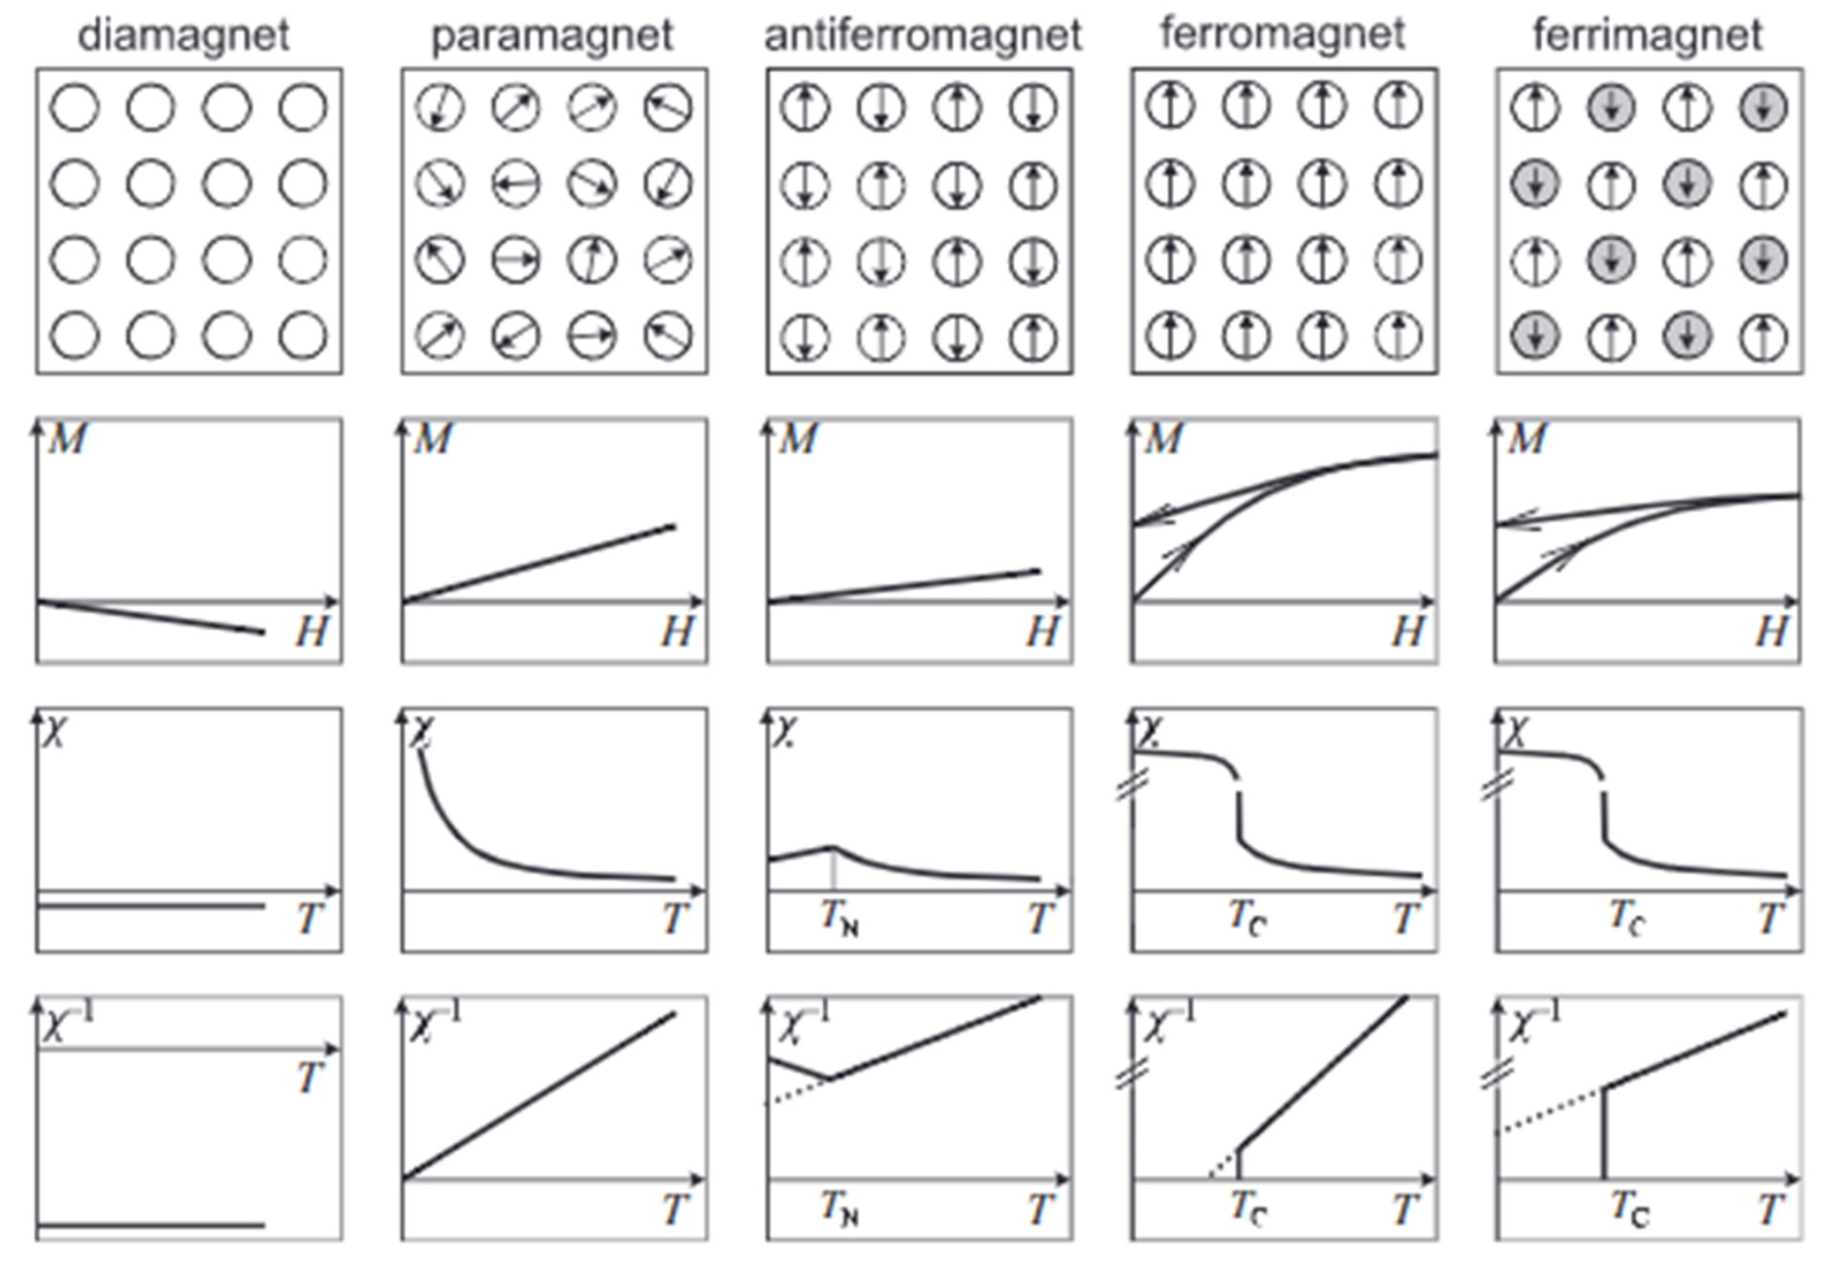
\includegraphics[width=0.65\linewidth]{bulkCoupling.png}
        \caption{Bulk magnetic coupling.}
        \label{fig:bulkCoupling}
    \end{table}
    \begin{itemize}
        \item Paramagnets have a bunch of spins with no preference for alignment. Note that $1/\chi$ is linear as discussed last lecture!
        \item Ferromagnet: We would need thermal energy to break the paired spins. This is an unstable equilibrium.
        \item Ferrimagnet: Closer to an antiferromagnet theoretically. Treats alloys where we have oppositely aligned differing spin populations. Behavior is almost exactly ferromagnetic.
    \end{itemize}
    \item \textbf{Pauli paramagnetism}: A metal that's a pool of electrons which are sloshing around in a band structure. Pool of positive and negative spins. Treat it as an electron gas. Applying a magnetic field changes the relative energies of the pool or electrons.
    \begin{figure}[h!]
        \centering
        \begin{tikzpicture}
            \begin{scope}
                \draw [blx,thick,name path=well]
                    (0,0) parabola (-1,1.8)
                    (0,-1) -- (0,2)
                    (0,0) parabola (1,1.8)
                ;
    
                \path [name path=int] (-1,1.3) -- ++(2,0);
                \begin{scope}[on background layer]
                    \fill [blz,name intersections={of=int and well}]
                        (0,0) parabola (intersection-1) -- (intersection-2) -- cycle
                        (0,0) parabola (intersection-3) -- (intersection-2) -- cycle
                    ;
                \end{scope}
                \node at (-0.48,1.6) {\Large$\upharpoonleft$};
                \node at (0.48,1.6) {\Large$\downharpoonright$};
            \end{scope}
            \draw [very thick,-latex] (1.5,0.5) -- ++(2,0);
            \begin{scope}[xshift=5cm]
                \draw [blx,thick,name path=well]
                    (0,0) parabola (-1,1.8)
                    (0,-1) -- (0,2)
                    (0,-0.2) parabola (1,1.8)
                ;
    
                \path [name path=int] (-1,1.3) -- ++(2,0);
                \begin{scope}[on background layer]
                    \fill [blz,name intersections={of=int and well}]
                        (0,0) parabola (intersection-1) -- (intersection-2) -- cycle
                        (0,-0.2) parabola (intersection-3) -- (intersection-2) -- cycle
                    ;
                \end{scope}
                \node at (-0.48,1.6) {\Large$\upharpoonleft$};
                \node at (0.48,1.6) {\Large$\downharpoonright$};
            \end{scope}
        \end{tikzpicture}
        \caption{Pauli paramagnetism.}
        \label{fig:pauliParamag}
    \end{figure}
    \begin{itemize}
        \item We now have more spin down, creating a net magnetic field that will be very small. \emph{This} is Pauli paramagnetism.
    \end{itemize}
    \item \ce{NdFeB} is the strongest \textbf{hard} ferromagnet.
    \item The most classic case of a ferrimagnet is magnetite (mixed \ce{Fe^2+} and \ce{Fe^3+}).
    \item Ferromagnets ideally have only one magnetic domain.
    \begin{figure}[h!]
        \centering
        \begin{tikzpicture}[
            every node/.style=black
        ]
            \begin{scope}
                \filldraw [draw=orx,fill=orz,thick] (-0.5,-0.7) rectangle node{\Large$\uparrow$} ++(1,1.4);
            \end{scope}
            \draw [very thick,-latex] (0.9,0) -- ++(1.2,0);
            \begin{scope}[xshift=3cm]
                \filldraw [draw=orx,fill=orz,thick] (-0.5,-0.7) rectangle node{\Large$\uparrow$} ++(0.5,1.4);
                \filldraw [draw=orx,fill=rez,thick] (0,-0.7) rectangle node{\Large$\downarrow$} ++(0.5,1.4);
            \end{scope}
            \draw [very thick,-latex] (3.9,0) -- ++(1.2,0);
            \begin{scope}[xshift=6cm]
                \filldraw [draw=orx,fill=orz,thick] (-0.5,-0.7) rectangle node{\Large$\uparrow$} ++(0.5,1.4);
                \filldraw [draw=orx,fill=rez,thick] (0,-0.7) rectangle node{\Large$\downarrow$} ++(0.5,1.4);
                \filldraw [draw=orx,fill=ylz,thick] (-0.5,-0.7) -- node[above=-1.5pt]{$\leftarrow$} ++(1,0) -- ++(-0.5,0.4) -- cycle;
                \filldraw [draw=orx,fill=ylt,thick] (-0.5,0.7) -- node[below=-1.5pt]{$\rightarrow$} ++(1,0) -- ++(-0.5,-0.4) -- cycle;
            \end{scope}
        \end{tikzpicture}
        \caption{Ferromagnetic domains.}
        \label{fig:FMdomains}
    \end{figure}
    \begin{itemize}
        \item Over time, under different magnetic fields, you'll get fracturing domains. These may align antiparallel.
        \item Applying a strong external magnetic field can anneal the domain walls and get you back to a single domain.
    \end{itemize}
    \item \textbf{Saturation magnetization}: The maximal magnetization of a material. \emph{Denoted by} $\bm{M_\textbf{sat}}$.
    \item \textbf{Remnant magnetization}: The magnetization of a magnetized material after the external field is dialed back. \emph{Denoted by} $\bm{M_\textbf{rem}}$.
    \item \textbf{Coercive field}: The amount of external field required to flip a magnet. \emph{Denoted by} $\bm{H_C}$.
    \item Visualizing $M_\text{sat}$, $M_\text{rem}$, and $H_C$.
    \begin{figure}[h!]
        \centering
        \begin{tikzpicture}
            \small
            \draw
                (-2,0) -- (2,0) node[right]{$H$}
                (0,-2) -- (0,2) node[above]{$M$}
            ;
    
            \footnotesize
            \draw [rex,thick] (1.6,1.6) node[circle,fill,inner sep=1.5pt,label={above right:${\color{black}M_\text{sat}}$}]{}
                to[out=180,in=10,looseness=0.5] (0,1.5) node[circle,fill,inner sep=1.5pt,label={below right:${\color{black}M_\text{rem}}$}]{}
                to[out=-170,in=90] (-0.9,0) node[circle,fill,inner sep=1.5pt,label={below left:${\color{black}H_C}$}]{}
                to[out=-90,in=0] (-1.6,-1.6)
                to[out=0,in=-170,looseness=0.5] (0,-1.5)
                to[out=10,in=-90] (0.9,0)
                to[out=90,in=180] cycle
            ;
        \end{tikzpicture}
        \caption{Hysteresis loop.}
        \label{fig:hysteresis}
    \end{figure}
    \begin{itemize}
        \item $H_C\propto\text{SOC}$, i.e., spin-orbit coupling.
        \item Things like \ce{Fe^3+} HS $d^5$ with equally (singly) occupied $d$ orbitals have no preferred orientation.
        \begin{itemize}
            \item \ce{Ti^3+} with $d^1$ can generate "ring currents," giving it a preferred orientation.
        \end{itemize}
        \item The wider the curve, the \textbf{harder} the ferromagnet.
        \item \textbf{Soft} is much skinnier (good for things like transformers that you want to be able to switch).
        \item To mediate coupling between $f$ orbitals in lanthanides, we mix in a bit of iron to use its free electrons.
    \end{itemize}
    \item Exotic things just to be aware of.
    \begin{itemize}
        \item Ferrometals: Iron is an example.
        \begin{itemize}
            \item Metallic band structure even in the absence of a magnetic field.
        \end{itemize}
        \item Ferro half metal.
        \begin{itemize}
            \item Charge carriers are spin-polarized.
            \item Important in spin-tronic type applications, P/N junctions, etc.
        \end{itemize}
        \item Metals have a continuous set of bands at the Fermi level regardless.
        \item Ferro insulator.
        \begin{itemize}
            \item Filled band with no density of states. A magnet that is not conductive, essentially.
        \end{itemize}
        \item Weak coupling or frustration. AF exchange with spins that get frozen in. Frustration: Triangular lattice with up/down/what's the third.
        \item Spin glass: Freeze-in spin orientations such that when you get back to a certain magnetization, you auto-drop.
    \end{itemize}
    \item Magnetic properties of some anonymized commercial polycrystalline hard magnets.
    \item Next week: EPR.
\end{itemize}




\end{document}